\documentclass[a4paper,11pt]{book}

\usepackage{hyperref}
%\usepackage{xspace}
\usepackage[T1]{fontenc}
%\usepackage{palatino}
% \usepackage[dvips,dvipdf]{graphics}
\usepackage{graphics}
\usepackage{epsfig}
\usepackage{url}
\usepackage{a4wide}
%\usepackage{boxedminipage}
%\usepackage{calc}
\usepackage{fancybox}
\usepackage{alltt}
%\usepackage{moreverb}
\usepackage{longtable}
\usepackage{array}
\usepackage{color}
%\usepackage{rotating}
%\usepackage{sectionbox}
\usepackage{listings}
% \usepackage{ae}
% \usepackage{aecompl}
% \usepackage[cm]{aeguill}
% \usepackage{times}
% \usepackage{bookman}
\usepackage{palatino}
\usepackage{verbatim}

\sloppy
\newcommand{\version}{0.1}

\newcommand{\code}[1]{{\tt{#1}}}

\newcommand{\note}[1]{\textbf{Note: }\textit{#1}}

\bibliographystyle{plain}

\title{\textbf{\Huge AKANTU}\\
  \vspace{0.5cm}
  \textbf{\huge User's Guide}\\
  \vspace{1cm}
  {\small \today{} --- Version \version}
}

\date{}

\begin{document}

\maketitle

\tableofcontents

\chapter{Introduction}

\section{Data structures\label{chap:data-structure}}

\subsection{Vectors\label{sec:vectors}}

The Vector class is a template class  that can store scalar types as Real, UInt,
Int  or bool.   A Vector  instance is  defined  by its  size and  its number  of
component.  It also  has an  identifier and  some extra  internal  variables for
memory handling purpose.

\begin{itemize}
\item The size is the number of tupels stored in the Vector.
\item The number of component is the number of values stored for each tuple.
\end{itemize}

\begin{figure}[!htb]
  \centering
  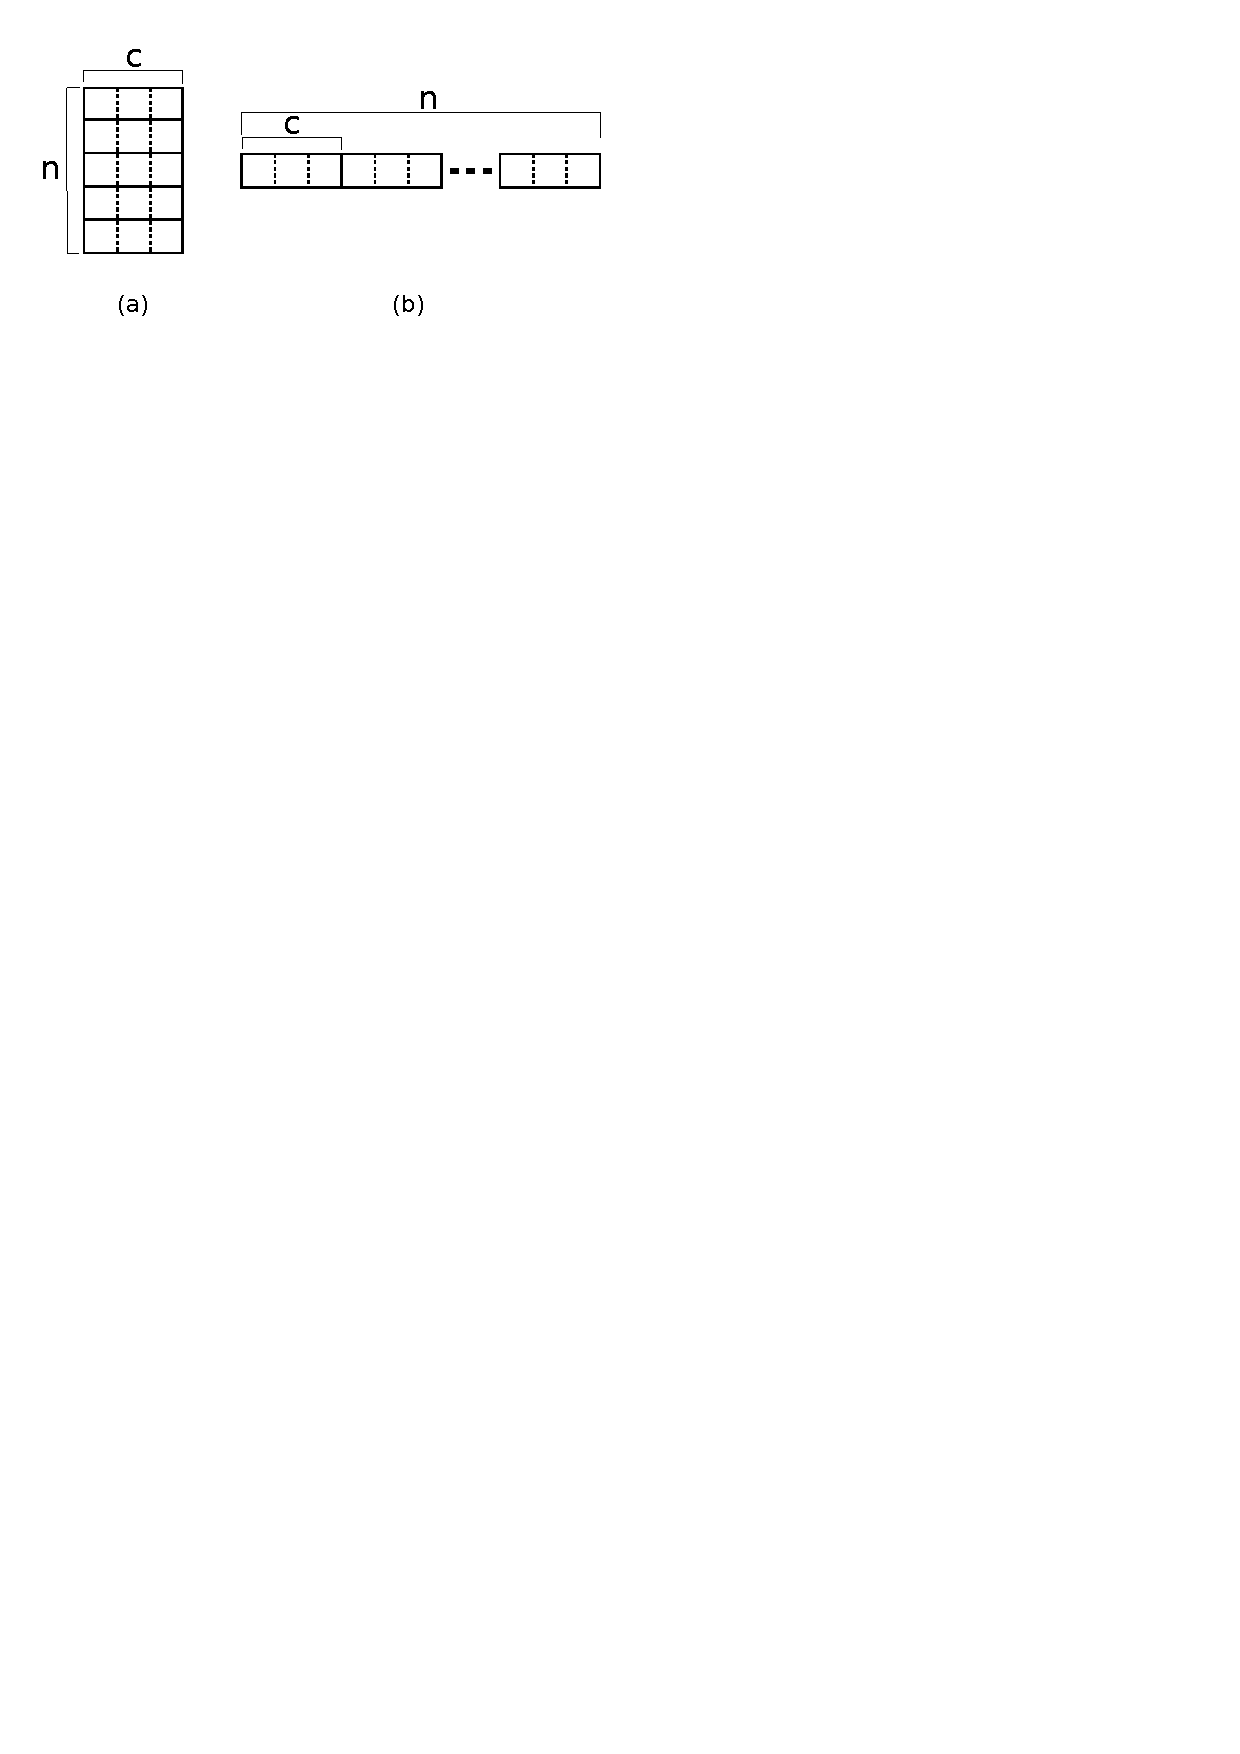
\includegraphics{figures/vectors}
  \caption{View of  a Vector of size  n and c compenents,  (a) representation of
    the vector, (b) representation of the storage of the same Vector.}
  \label{fig:vectors}
\end{figure}

All the  data are linerarized  in memory in  an array called values.  This class
member is public.  So for a Vector  of size $n$ and $c$ component, to access the
$j^{th}$  component of  th  $i^{th}$ tuple,  you have  to  get $values[i  * c  +
j]$. You  can also  access to this  value with  accessor \code{at(i, j)}  or the
constant accessor \code{get(i, j)}.

If  you want to  store a  matrix on  each tuple  you have  to linearize  it. For
exemple if you want to store a m * k matrix on each tuple you must specify c = m
* k.  To access a particular value  in a matrix of  a tuple you will  have to do
something like $values[ i * m * k + j_i * m + j_j]$.

\subsubsection{Vector storage convention within FE object\label{sec:FE-convention}}

The point of  this section is to describe the convention  of storage for vectors
intented  to be  passed to  {\bf  FE} object  methods.  Indeed  a convention  of
necessary  since gradient  operators or  integrtaion loops  will use  vectors as
input and ouput.   Such vectors will be ordered with  a specific convention that
we intend to describe now.

For  vector objects,  the  size of  the vector  is  always the  number of  nodes
associated.  The number  of components  is related  to the  order of  the tensor
considered. For a scalar  field it is 1, for a vectorial  field, the size of the
vector is the number of components. For a $m\times n$ matrix field the number of
components is $m\times n$.

One common operation  is the manipulation of continuum  fields at the quadrature
point  positions.   Here  the  size   of  the  vector  is   $mn\_element  \times
nb\_quad\_points$  and  the  number  of  components is  related  to  the  stored
object.  For instance the  method \verb$interpolateOnQuadraturePoints()$  take a
nodal field  stored in a  vector($n\_nodes$,$dim$) and return  a vector($n\_elem
\times n\_quads$,$dim$).

Basic gradient operations, like method \verb$gradientOnQuadraturePoints()$, will
take  as input a  vector($n\_nodes$,$dim$) and  return a  vector($n\_elem \times
n\_quads$,$dim \times spatial\_dimension$) where spatial dimension is the number
of dimension in which the domain is embedded.

In  the  same  way   the  integration  routines  expect  vector($n\_elem  \times
n\_quads$,$dim$)  and  will  return vector($n\_elem$,$dim$).   For  non-Gaussian
integrations, the input  by be direction a nodal field.   (At present time, only
gaussian integrators are implemented within akantu).

Last but  not the least  is the vectorial  assembly process for which  accept as
input vector($n\_elem \times n\_quads \times n\_nodes\_per\_element$,$dim$)
and will return a vector($n\_nodes$,$dim$) nodal object.\\

{\bf The general convention is that  the number of component shall always be the
  size of  the object manipulated  at the lowest  level.  The object could  be a
  per-element, of  per quadrature point  or even per  node basis this  will also
  apply    as   shown    below.   The    figures    \ref{fig:vector-chain}   and
  \ref{fig:interpolate-storage} shows the  pattern of the vectors is  the case a
  interpolation on quadrature points.}

\begin{figure}
  \begin{equation}
    \left(
      \begin{array}{c}
	N_1 \\
	\vdots \\
	N_I
	\left\{
	  \begin{array}{c}
	    a_1 \\
	    \vdots \\
	    a_{dim} \\
	  \end{array}
	\right. \\
	\vdots \\
	N_{nb\_nodes}
      \end{array}
    \right)
    \begin{array}{c}
      \Longrightarrow \\
      interpolate\\
      On\\
      Quadrature\\
      Points\\
    \end{array}
    \left(
      \begin{array}{c}
	E_1 \\
	\vdots \\
	E_e
	\left\{
	  \begin{array}{c}
	    q_1 \\
	    \vdots \\
	    \left.
	      \begin{array}{c}
		a_1 \\
		\vdots \\
		a_{dim}
	      \end{array}
	    \right\} q_i \\
	    \vdots \\
	    q_p \\
	  \end{array}
	\right.  \\
	\vdots \\
	E_{nb\_elements}
      \end{array}
    \right)
  \end{equation}
  \caption{\label{fig:vector-chain}Pattern   of   vectors   manipulated   during
    interpolation on  quadrature points.  Symbols  N (resp. E, q)  denotes nodes
    (resp. elements, quadrature points).}
\end{figure}

\begin{figure}[!htb]
  \centering
  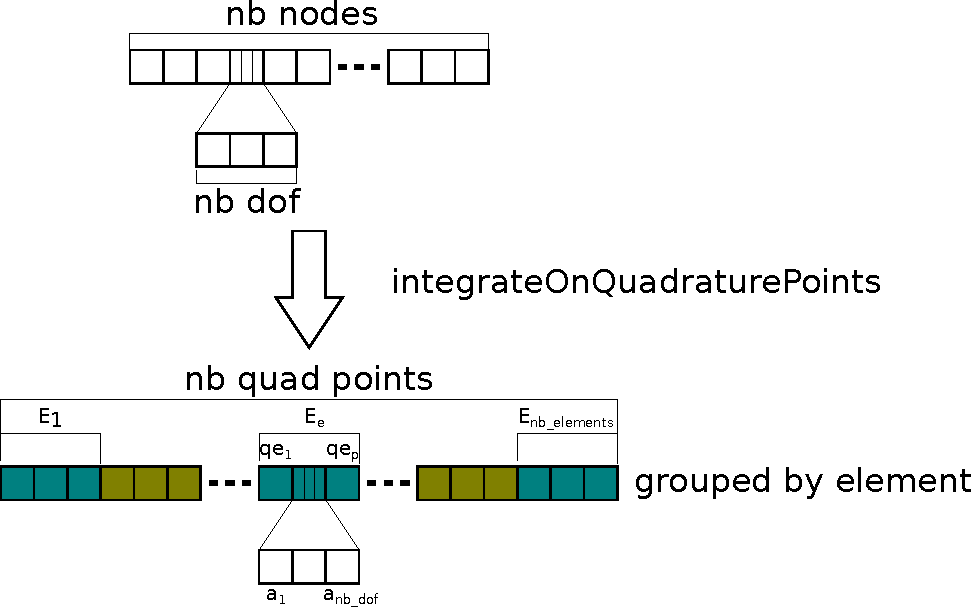
\includegraphics[width=\textwidth]{figures/interpolate}
  \caption{Input and output  vector of interpolateOnQuadraturePoints. The output
    Vector has nb\_quadrature\_points tuples,  the quadrature points are grouped
    by elements (p is the number of quadrature points per element).}
  \label{fig:interpolate-storage}
\end{figure}


\chapter{How to use Akantu}
\section{Getting start}
\subsection{Downloading the code}
SVN URL to get akantu :

\noindent {\small\code{svn co

  svn+ssh://username@intranet-lsms.epfl.ch/space/repositories/SimulPack/akantu/trunk akantu}}

% or via http:

% \noindent {\small\code{svn co

%   http://username@intranet-lsms.epfl.ch/svn/akantu/trunk/ akantu}}

\subsection{Compiling akantu}
\noindent\code{> mkdir build}

\noindent\code{> cd build}

\noindent\code{> ccmake <path to akantu sources>}

Set the option that you need

\noindent\code{> make}

\noindent\code{> make install}


\section{Solid Mechanics model}

The  solid  mechanics  model  is   a  specific  implementation  of  the  model
interface. The model is instantiated for a given mesh. It will create is own FEM
object   to   do  the   interpolation,   gradient,   integration  and   assemble
operations. This model contain some Vectors that we will describe now.

\begin{description}
\item[Displacement] contain the displacements of  the free degrees of freedom or
  the imposed displacements for the blocked degrees of freedom.
\item[Velocity] contain the velocities of  the degree of freedoms, acts like the
  displacement vector
\item[Acceleration] contain  the accelerations of  the degree of  freedoms, acts
  like the displacement vector
\item[Force] contain the external forces applied on the different nodes.
\item[Residual] contain the difference  between external and internal forces. On
  blocked degree of freedom, residual contain the reactions form the support.
\end{description}

We will present more in detail through some examples how to use this model.

\subsection{Set up a model}
\subsubsection{Create and load a mesh}


\begin{verbatim}
  UInt spatial_dimension = 2;

  Mesh mesh(spatial_dimension);

  MeshIOMSH mesh_io;
  mesh_io.read("square.msh", mesh);
\end{verbatim}

\subsubsection{Set initial conditions}
\subsubsection{Set boundary conditions\label{sect:smm:boundary}}

\begin{verbatim}
  const  Vector<Real> & position = mesh.getNodes();
  Vector<bool> & boundary = model.getBoundary();
  Vector<Real> & displacment = model.getDisplacement();

  for (UInt n = 0; n < nb_nodes; ++n) {
    if(position(n,0) < Math::getTolerance()) boundary(n,0) = true;
    if(position(n,1) < Math::getTolerance()) boundary(n,1) = true;

    if(std::abs(position(n,0) - bar_length) < Math::getTolerance()) {
      boundary(n,0) = true;
      displacment(n,0) = 0.1;
    }
  }
\end{verbatim}

This conditions put the left and bottom side on rollers

\subsection{Resolution methods}
In the  solid mechanics  model different  way to solve  the motion  equation are
implemented.  The equations  to  solve is  mainly  $Ma +  Cv +  Ku  = f_{ext}  -
f_{int} = q$. So we can solve static case where $a = v = 0$, for this we only need a
solver, like Mumps(\cite{mumps}) for example.

We  can also  solve  the complete  equation,  and for  this we  can  do it  with
different time discretizations, either  explicit or implicit.  By default Akantu
use  a  predictor-corrector  Newmark-$\beta$  time integration  scheme.

So the three differentiate equations (dynamic and cinematic) are \cite{curnier92a}:
\begin{eqnarray}
  M \ddot{u}_{n+1} + C \dot{u}_{n+1} + K u_{n+1} &=& q_{n+1} \\
  u_{n+1} &=& u_{n} + (1 - \alpha) \Delta t \dot{u}_{n} + \alpha \Delta t \dot{u}_{n+1} + (1/2 - \alpha) \Delta t^2 \ddot{u}_n \\
  \dot{u}_{n+1} &=& \dot{u}_{n} + (1 - \beta) \Delta t \ddot{u}_{n} + \beta \Delta t \ddot{u}_{n+1}
\end{eqnarray}

can be rewrote as

\noindent Predictor:
\begin{eqnarray}
  u^{0}_{n+1}        &=& u_{n} +  \Delta t \dot{u}_n + \frac{\Delta t^2}{2} \ddot{u}_n \\
  \dot{u}^{0}_{n+1}  &=& \dot{u}_{n} +  \Delta t \ddot{u}_{n} \\
  \ddot{u}^{0}_{n+1} &=& \ddot{u}_{n}
\end{eqnarray}

\noindent Solve :
\begin{eqnarray}
 (c M + d C + e K^i_{n+1}) w = q_{n+1} - f^i_{n+1} - C \dot{u}^i_{n+1} - M \ddot{u}^i_{n+1}
\end{eqnarray}

\noindent Corrector :
\begin{eqnarray}
  \ddot{u}^{i+1}_{n+1} &=& \ddot{u}^{i}_{n+1} + c w \\
  \dot{u}^{i+1}_{n+1} &=& \dot{u}^{i}_{n+1} + d w \\
  u^{i+1}_{n+1} &=& u^{i}_{n+1} + e w
\end{eqnarray}

c, d and e are parameters depending on the method used to solve the equations

\begin{center}
  \begin{tabular}{l|c|c|c|c}
    & w & e & d & c\\
    \hline
    in acceleration &$ \delta \ddot{u}$ & $\alpha \beta \Delta t^2$ &$\beta \Delta t$ &$1$\\
    in velocity & $ \delta \dot{u}$& $1/\beta \Delta t$ & $1$ & $\alpha \Delta t$\\
    in displacement &$\delta u$ & $ 1$ & $1/\alpha \Delta t$ & $1/\alpha \beta \Delta t^2$
  \end{tabular}
\end{center}

\note{In you want to use the  implicit solver Akantu should be compiled at least
  with one sparse matrix linear system solver.}

\subsubsection{Implicit static\label{sect:smm:implicit:static}}
The example presented here is \code{example/manuel/implicit\_static.cc}

The example is composed of a 2D  plate of steel blocked with rollers on the left
and bottom side as shown on figure \ref{fig:smm:implicit:static}. The nodes from
the right side  of the sample are  displaced from $10\%$ (since it  is a elastic
material, it can handle such a deformation).

\begin{figure}[!htb]
  \centering
  \includegraphics{figures/implicit_static}
  \caption{Numerical setup\label{fig:smm:implicit:static}}
\end{figure}

To  solve  this  problem  we  will   use  the  static  implicit  solver  of  the
SolidMechanicsModel object in Akantu. The following lines of code are an extract
of the example code.

\begin{verbatim}
  ...

1.  SolidMechanicsModel model(mesh);
2.  model.initFull("material.dat", true, false);

  ...

3.  model.assembleStiffnessMatrix();
4.  model.updateResidual();

5.  Real norm;
6.  UInt count = 0;
7.  while(!model.testConvergenceResidual(1e-3, norm) &&
8.        (count < 100)) {
9.    if (prank == 0)
10.      std::cout << "Iter : " << ++count
11.                << " - residual norm : "
12.                << norm << std::endl;
13.    model.solveStatic();
14.    model.updateResidual();
15. };
\end{verbatim}

The  part presenting  how to  create a  mesh and  read it  in Akantu  as already
presented before so here we skip this first part.

Once we have a  mesh we can use it to create  a SolidMechanicsModel object (line
1). This object need to be initialized in order to be used. In this case we want
to  initialize the  implicit solver.   For  this we  use the  initFull (line  2)
function that  initialize all the part  of the model. The  parameters are, first
the material file, and then 2 switches specifying that we need a implicit solver
not for dynamic case.

Once we  have the model  initialized we  can start to  use it. The  part skipped
between lines 2 and 3 corresponds  to the boundary conditions setup to in detail
how to set them check the section \ref{sect:smm:boundary}

What we want to solve is $Ku = f_{ext} - f_{int}$, so first we will assemble the
stiffness matrix $K$ (line 3), and then the second member $f$ (line 4).

The lines 5 to 15 correspond  to a Newton-Raphson convergence loop. In this case
this loop  is not needed since the  material is elastic. The  solution should be
found at  the first iteration.  So technically this  10 lines can replaced  by a
simple call to the \code{solveStatic} function.

The solution can be found in the displacement vector.


\subsubsection{Implicit dynamic}
The example presented here is \code{example/manuel/implicit\_dynamic.cc}

This example consists in a beam blocked on one side and on a roller on the other
side,  on  which   we  apply  a  constant  force  in   the  middle.  The  figure
\ref{fig:smm:implicit:dynamic} present the geometry of this case.

We can give a approximation  (eqn. \ref{eqn:smm:implicit}) of the dynamic answer
of the middle point of the beam.

\begin{equation}
  u(\frac{L}{2}, t) = \frac{1}{\pi^4} (1 - cos(\pi^2 t) +
  \frac{1}{81}(1 - cos(3^2 \pi^2 t)) +
  \frac{1}{625}(1 - cos(5^2 \pi^2 t)))
\end{equation}
\label{eqn:smm:implicit}

\begin{figure}[!htb]
  \centering
  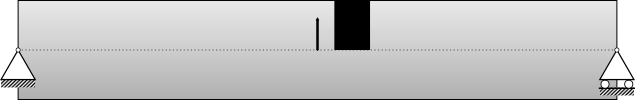
\includegraphics[scale=.6]{figures/implicit_dynamic}
  \caption{Numerical setup}
  \label{fig:smm:implicit:dynamic}
\end{figure}


\begin{verbatim}
   ...

1.  model.assembleStiffnessMatrix();
2.  model.assembleMass();

3.  model.setTimeStep(time_step);
    /// time loop
4.  for (UInt s = 1; time < 0.62; ++s) {

5.    model.implicitPred();

      /// convergence loop
6.    count = 0;
7.    do {
8.      if(count > 0)
9.        std::cout << "step " << s << " " << count++ << " : "
		    << std::scientific << error << "\r" << std::flush;

10.     model.updateResidual();
11.     model.solveDynamic();

12.     model.implicitCorr();
13.    } while(!model.testConvergenceIncrement(1e-12, error) &&
	       (count < 100));

14.    std::cout << "step " << s << " - " << count << " : "
		 << std::scientific << error << std::endl;

15.    pos << s << "," << s * time_step
	   << "," << displacment(node_to_print, 1)
	   << "," << analytical_solution(s*time_step) << std::endl;

16.    time += time_step;
17. }
\end{verbatim}

For  this simulation  everything  is really  similar  to the  example in  static
(section  \ref{sect:smm:implicit:static}) except  that  in this  one during  the
initialization of the model we have to specify that it is a dynamic case.

The difference here is that the equation we solve is now $Ma + Cv + Ku = f_{ext}
- f_{int}$. So we first have to  assemble the stiffness matrix $K$ (line 1) then
the mass matrix $M$ (in case of an elastic material $C = 0$).

\note{Here we have a elastic material so $K$ is constant, but for other material
  we should assemble $K$ at each iteration.}

Once the matrix assembled  we can start the time loop. To do  this we will use a
predictor-corrector  scheme. By  default  for  an implicit  resolution  it is  a
Newmark-$\beta$ in  the particular case of  the trapezoidal rule that  is to say
$\beta = 1/2$ and $\alpha = 1/2$.  The call to the predictor can be seen line 5,
and the corrector call is in the Newton-Raphson loop (line 12)

After the predictor we can solve the system to get the new displacement for this
time step. In these case  the Newton-Raphson convergence algorithm is needed due
to  non-linearity  potentially  introduced  the  dynamic  behavior.  The  motion
equation  in this  case  is solved  in  increment of  displacement,  so for  the
convergence criteria  we just have  to check that  the norm of the  increment of
displacement is smaller that a give threshold, here $10^{-12}$ (line 13).

\note{For the convergence loop  it is a good usage to put  also a limit in terms
  of number of iterations to avoid an  infinite loop in case of a error criteria
  to hard to reach.}

\subsubsection{Explicit}

\subsection{Constitutive laws}
\subsubsection{Elastic}
\subsubsection{Caughey}
\subsubsection{Neo-hookean}
\subsubsection{Visco-elastic}
\subsubsection{Damage Marigo}
\subsubsection{Damage Mazars}

\subsection{Adding a new constitutive law}

\subsection{Contact}

\subsection{Cohesive laws}


\section{Structural Mechanics model}

\section{Heat Transfer model}

% \subsection{Contact Neighbor Structure}

% The contact neighbor  structure is an interface which is  ment to be heritated
% from in order  to implement different type of  contact neighbor structures. It
% has the following protected attributes:
% \begin{itemize}
%   \item id
%   \item contact search
%   \item master surface
%   \item neighbor list
%   \item type
% \end{itemize}
% The \emph{id} and the \emph{type}  are characteristics of the contact neighcor
% structure object which  define its id and its  type. The \emph{contact search}
% attribute  is  the associated  contact  search  object  to the  given  contact
% neighbor structure  object. The \emph{master  surface} attribute is the  id of
% the  associated master  surface for  which the  neighbor structure  has  to be
% built. Finally, the neighbor list  is the constructed neighbor structure which
% defines the  impactor nodes  that are  in the neighborhood  of either  a given
% master  node or  a given  master  surface element,  depending on  the type  of
% contact neighbor structure.

% The contact neighbor structure provides the accessor \emph{getNeighborList} to
% the constructed  neighbor list and forces  the heritated classes  to provide a
% public \emph{initNeighborStructure}  function, which initializes  the neighbor
% structure,  as well  as a  public  \emph{update} function,  which updates  the
% neighbor structure.

% \subsubsection{Regular Grid Neighbor Structure}

% The regular  grid neighbor structure builds  a regular grid  around the master
% surface and  uses it in  order to construct  the neighbor list.  This neighbor
% structure can construct both types of neighbor list, the


% \subsection{Implementation of a new solid mechanics problem}

% Let us imagine you want to implement a new material called
% "toto" in akantu. The have to complete the following steps (in
% any order) :
% \begin{enumerate}
% \item
% Declare a new material in the file
%      \textit{Akantu/model/solid\_mechanics/solid\_mechanics\_model\_material.cc}.
% You have to had this line after the list of possible cases
% \begin{verbatim}else if(mat\_type == "toto") material =
%      parser.readMaterialObject<MaterialToto>(*this,mat_id);
% \end{verbatim}


% \item
% Include the new material in \textit{Akantu/model/solid\_mechanics/material.hh} \\
% add the line :
% \begin{verbatim}
% #include "materials/material\_toto.hh"
% \end{verbatim}

% \item
% For compilation include the new file to compile in
%      \textit{Akantu/CMakelist.txt} by adding
% \begin{verbatim}
% model/solid_mechanics/materials/material_toto.cc
% \end{verbatim}
% \item
% In \textit{Akantu/model/solid\_mechanics/materials}, create (or copy from
%      an allready existing material) the three following files :\\
% - material\_toto.cc\\
% - material\_toto.hh\\
% - material\_toto\_inline\_impl.cc

% \item
% Modify the files !

% \end{enumerate}
\bibliography{biblio}



\end{document}
